% Standalone figure: the agentic quiz-generation loop.
%
% Build:  lualatex -output-directory=figs figs/agentic-loop.tex
% Included by poster.tex as figs/agentic-loop.pdf
%
% Journal conventions used here: restrained palette, hairline rules, one accent
% colour per semantic role, no gradients or drop shadows, every arc labelled,
% and the failure paths visually subordinate (dashed, thinner) to the main path.
% Each remediation re-enters the pipeline at a DIFFERENT stage, so each gets its
% own return bus at a distinct x offset -- overlapping arcs make routing
% unreadable, which is the usual failure of this kind of figure.
%
% Two-line node labels go through \stg, which uses a tabular. A bare \\ inside a
% tikz node is fragile here; tabular's row break is not.
\documentclass[border=8pt]{standalone}

\usepackage[T1]{fontenc}
\usepackage{lmodern}
\usepackage{xcolor}
\usepackage{tikz}
\usetikzlibrary{arrows.meta, positioning, calc}

\definecolor{JInk}{HTML}{111827}
\definecolor{JLine}{HTML}{374151}
\definecolor{JBlue}{HTML}{1D4ED8}
\definecolor{JAmber}{HTML}{B45309}
\definecolor{JGreen}{HTML}{047857}
\definecolor{JRed}{HTML}{B91C1C}
\definecolor{JGrey}{HTML}{6B7280}

% title over muted caption, centred
\newcommand{\stg}[2]{%
  \begin{tabular}{@{}c@{}}
    \textbf{#1}\\[2pt]
    {\scriptsize\color{JGrey}#2}
  \end{tabular}}

\begin{document}
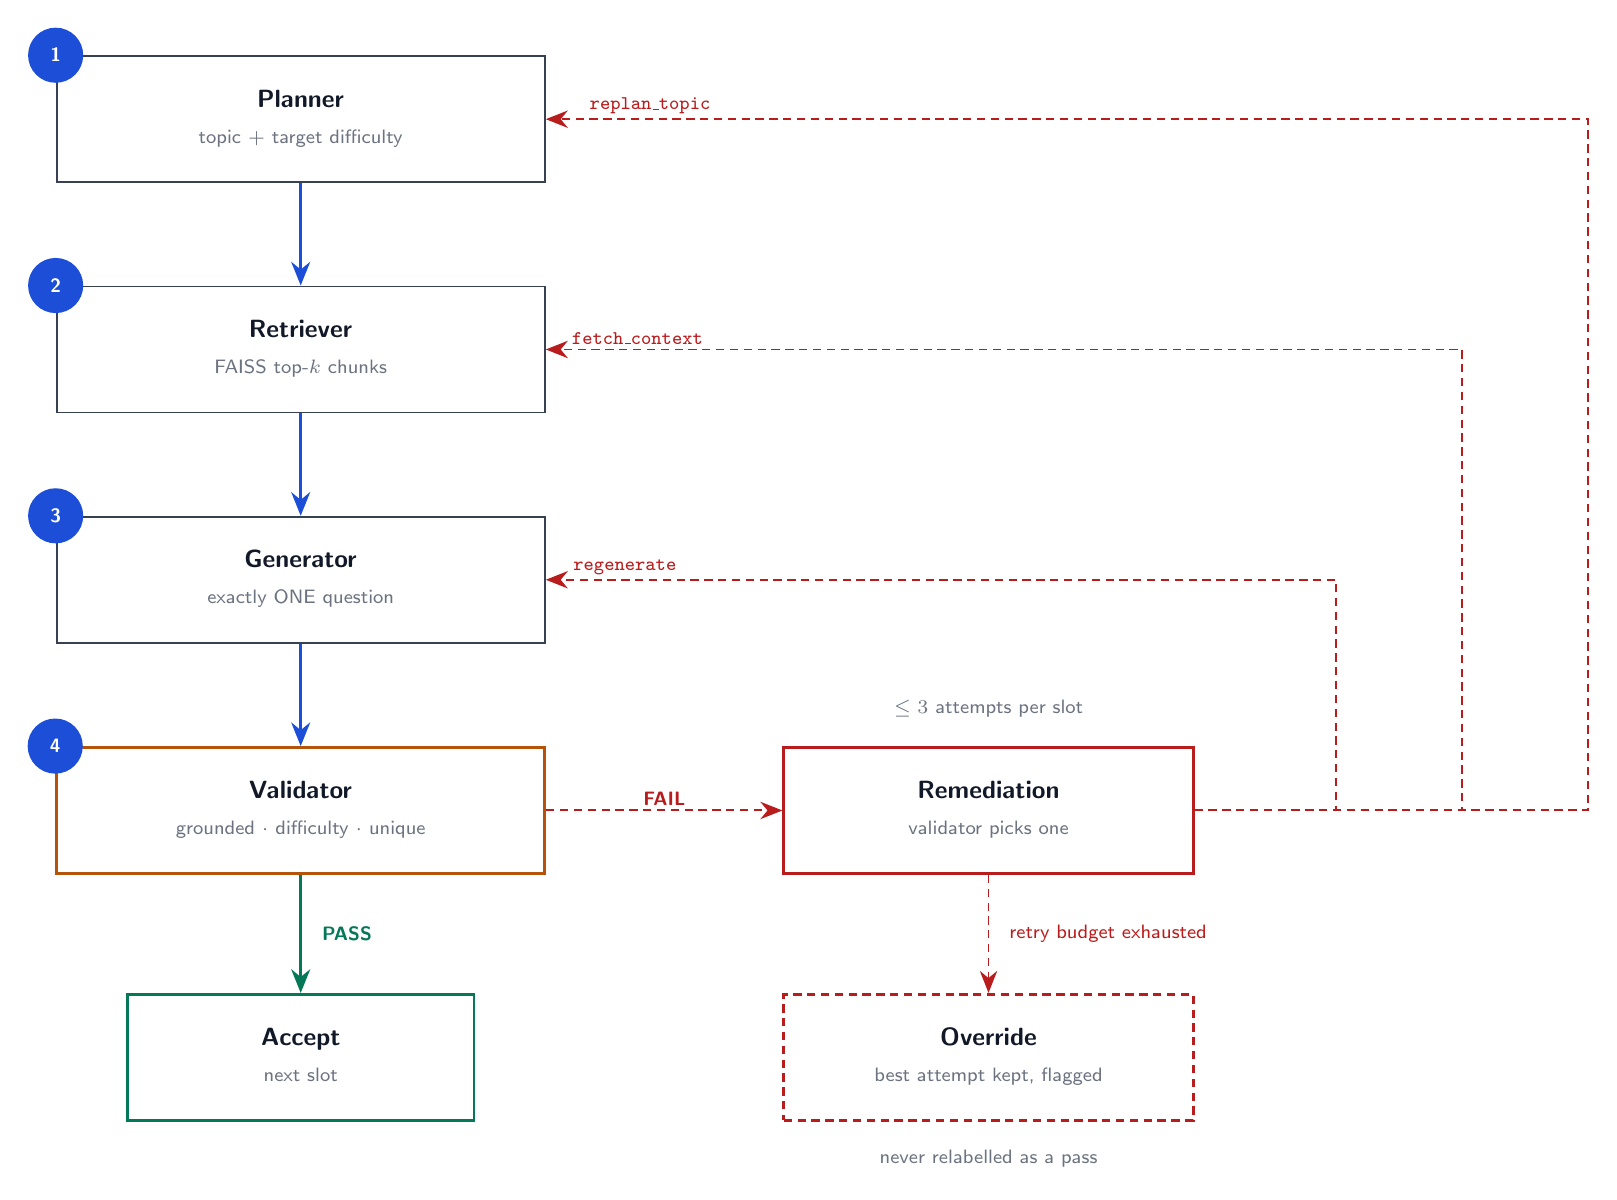
\begin{tikzpicture}[
  font=\sffamily\small,
  stage/.style={rectangle, draw=JLine, line width=0.7pt, fill=white,
                text=JInk, minimum width=62mm, minimum height=16mm,
                inner sep=3mm},
  decision/.style={stage, draw=JAmber, line width=1pt},
  accept/.style={stage, draw=JGreen, line width=1pt, minimum width=44mm},
  override/.style={stage, draw=JRed, line width=1pt, minimum width=52mm,
                   densely dashed},
  num/.style={circle, fill=JBlue, text=white,
              font=\sffamily\bfseries\scriptsize, inner sep=0pt,
              minimum size=7mm},
  flow/.style={-{Stealth[length=3mm,width=2.4mm]}, draw=JBlue, line width=1.1pt},
  pass/.style={-{Stealth[length=3mm,width=2.4mm]}, draw=JGreen, line width=1.1pt},
  fail/.style={-{Stealth[length=2.8mm,width=2.2mm]}, draw=JRed, line width=0.7pt,
               densely dashed},
  lbl/.style={font=\sffamily\scriptsize, inner sep=1.5pt},
]

% ── main vertical path ───────────────────────────────────────────────────
\node[stage]                     (plan) {\stg{Planner}{topic $+$ target difficulty}};
\node[stage, below=13mm of plan] (ret)  {\stg{Retriever}{FAISS top-$k$ chunks}};
\node[stage, below=13mm of ret]  (gen)  {\stg{Generator}{exactly ONE question}};
\node[decision, below=13mm of gen] (val)
  {\stg{Validator}{grounded $\cdot$ difficulty $\cdot$ unique}};

\draw[flow] (plan) -- (ret);
\draw[flow] (ret)  -- (gen);
\draw[flow] (gen)  -- (val);

\node[num] at (plan.north west) {1};
\node[num] at (ret.north west)  {2};
\node[num] at (gen.north west)  {3};
\node[num] at (val.north west)  {4};

% ── accept branch ────────────────────────────────────────────────────────
\node[accept, below=15mm of val] (acc) {\stg{Accept}{next slot}};
\draw[pass] (val) -- (acc)
  node[lbl, midway, right=2mm, text=JGreen] {\textbf{PASS}};

% ── remediation router ───────────────────────────────────────────────────
\node[stage, draw=JRed, line width=1pt, right=30mm of val, minimum width=52mm]
  (rem) {\stg{Remediation}{validator picks one}};
\draw[fail] (val) -- (rem)
  node[lbl, midway, above, text=JRed] {\textbf{FAIL}};

% Three return buses at distinct x offsets: innermost re-enters at the
% Generator, middle at the Retriever, outermost at the Planner.
\coordinate (b1) at ([xshift=18mm]rem.east);
\coordinate (b2) at ([xshift=34mm]rem.east);
\coordinate (b3) at ([xshift=50mm]rem.east);

\draw[fail] (rem.east) -- (b1) |- (gen.east)
  node[lbl, pos=0.95, above, text=JRed] {\texttt{regenerate}};
\draw[fail] (rem.east) -- (b2) |- (ret.east)
  node[lbl, pos=0.95, above, text=JRed] {\texttt{fetch\_context}};
\draw[fail] (rem.east) -- (b3) |- (plan.east)
  node[lbl, pos=0.95, above, text=JRed] {\texttt{replan\_topic}};

% ── budget exhaustion ────────────────────────────────────────────────────
\node[override, below=15mm of rem] (ovr)
  {\stg{Override}{best attempt kept, flagged}};
\draw[fail] (rem) -- (ovr)
  node[lbl, midway, right=2mm, text=JRed] {retry budget exhausted};

\node[lbl, below=3mm of ovr.south, text=JGrey] {never relabelled as a pass};
\node[lbl, above=3mm of rem.north, text=JGrey] {$\le 3$ attempts per slot};

\end{tikzpicture}
\end{document}
